%%%%%%%%%%%%%%%%%%%%%%%%%%%%%%%%%%%%%
% Read the /ReadMeFirst/ReadMeFirst.tex for an introduction. 
% Check out the accompanying book "Even Better Books with LaTeX the Agile Way in 2023" for a discussion of the template and step-by-step instructions. 
% The template was originally created by Clemens Lode, LODE Publishing (www.lode.de), 1/1/2023. Feel free to use this template for your book project!
% Contact me at mail@lode.de if you need help with the template or want editing and publishing services.
%%%%%%%%%%%%%%%%%%%%%%%%%%%%%%%%%%%%%


\chapter{Accompanying Book for the Template}\label{additional-titles:sec}

% Remove the following section if you only want to show your covers, replace it with your own book descriptions.

In \citetitle{eBBWLtAW}\index{@\citetitle{eBBWLtAW}}\ifxetex\else{} \citep{eBBWLtAW}\fi (\url{https://www.amazon.com/Even-Better-Books-LaTeX-Agile-ebook/dp/B0BMZJ5LF7}), author Clemens Lode provides you a short-cut into the world of book publishing with LaTeX. It is not a book that just lists all the commands and then leaves you alone, it guides you alongside a fully working template (this one!).

% If you do not have or want covers displayed here, comment them out.
\begin{center}
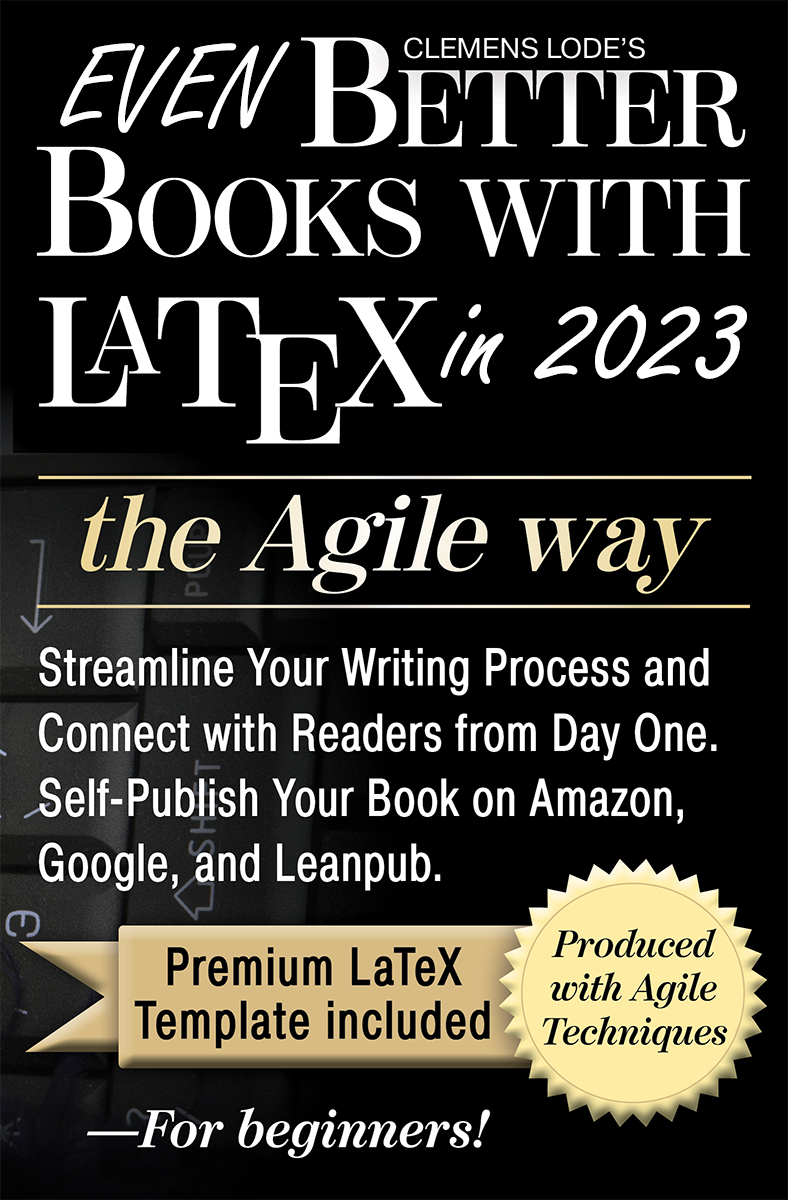
\includegraphics[width=.45\textwidth]{images/cover.jpg}
\end{center}

At LODE Publishing, we also publish works on science, philosophy, and project management. Check out \url{https://www.lode.de/publications} for a list. If you are interested in working with us to publish your book or advice you on the steps to take, contact us at \textbf{mail@lode.de}.